\section{Discussion} \label{sec:discussion} 
\subsection{Comparison to baseline approach}
Our baseline approach was the Delta Method described in Section
\ref{subsec:method:delta_method}. One of the goals of this report was finding
and implementing methods for authorship verification that could beat our
baseline method. An overview of the different methods final results can be seen
in Table \ref{tab:all_final_results}. We were able to beat
the baseline method both on the PAN 2013 dataset and the PAN 2015 dataset.

\begin{table}
    \centering
    \begin{tabular}{ll|cc}
        \textbf{Method}           &           & \textbf{PAN 2013} & \textbf{PAN 2015} \\ \hline
        Delta (BASELINE)          & Score     & 0.62252           & 0.34201           \\
                                  & \gls{TPR} & 0.52196           & 0.54899           \\
                                  & \gls{TNR} & 0.71204           & 0.60800           \\
                                  & Rank      & 13/19             & 10/17             \\ \hline
        Random Forest (\gls{UBM}) & Score     & n/a               & 0.38576           \\
                                  & \gls{TPR} & n/a               & 0.63200           \\
                                  & \gls{TNR} & n/a               & 0.57600           \\
                                  & Rank      & n/a               & 9/17              \\ \hline
        Random Forest (Minus)     & Score     & n/a               & 0.33183           \\
                                  & \gls{TPR} & n/a               & 0.66800           \\
                                  & \gls{TNR} & n/a               & 0.50000           \\
                                  & Rank      & n/a               & 10/17             \\ \hline
        Extended Delta            & Score     & 0.69909           & 0.40383           \\
                                  & \gls{TPR} & 0.71255           & 0.49760           \\
                                  & \gls{TNR} & 0.68098           & 0.74140           \\
                                  & Rank      & 10/19             & 8/17              \\ \hline
        Author Specific SVM       & Score     & 0.77858           & n/a               \\
                                  & \gls{TPR} & 0.71114           & n/a               \\
                                  & \gls{TNR} & 0.83582           & n/a               \\
                                  & Rank      & 3/20              & n/a
    \end{tabular}
    \caption{Final results for all our implemented algorithms on the test
        datasets of PAN 2013 and PAN 2015. Since there are two test datasets for
        PAN 2013 \textit{Score}, \textit{\gls{TPR}} and \textit{\gls{TNR}} in
        the PAN 2013 column are all an average over the values on the two
        datasets. Algorithms that were only made for one of the dataset has
        \textit{n/a} in the fields they are missing.}
    \label{tab:all_final_results}
\end{table}

\subsection{Comparison to other PAN results}
The best results for the PAN 2013 dataset can be found in Appendix
\ref{sec:appendix:pan_2013_results} and our results can be found in Table
\ref{tab:all_final_results}. We obtained the third best result out of 19
submitted results (excluding our own). The method we obtained the score with
was the author specific SVM. The best approach that beat our method was the
approach described by \cite{seidman:2013}. They used a \textit{GenIM} method
that uses the imposter method. To determine whether a document $X$ is written by
the same author as has written $Y$, $X$ is compared to $Y$ and to a random set
of imposter documents. If $X$ is found to be closer to $Y$ than the imposters
it is reported as written by the same author and not otherwise. The approach is
similar to ours as we also use text from other authors to do the verification.
However \cite{seidman:2013} did not use the training set as the set of imposters
but rather generated the imposters from data found on the internet. It might
be that the reason he performed better than we did was because he had a better
set of imposters. \cite{seidman:2013} also used predefined function words as
features. So instead of using only normal n-grams as we do they used prior
knowledge about the language to construct good features.

The other PAN 2013 method that achieved better results than we did is described
by \cite{veenman:2013}. Their method used the compression method of authorship
verification. They determine the authorship of a text by generating a set
of imposter texts and using the compression distance to see whether the
unknown text is closer to the known texts or to the imposter set. Like
\cite{seidman:2013} the imposter set is generated by using external text and
\cite{veenman:2013} even mention that the selection of the imposter set was an
important part of the solution. Again we might have been able to beat their
result if we had tried using external texts as our set of opposing authors.

The best results for the PAN 2015 dataset can be found in Appendix
\ref{sec:appendix:pan_2015_results} and our results can be found in Table
\ref{tab:all_final_results}. We obtained the 8'th place out of 17 submitted
results (excluding our own). The method that we used was the Extended Delta
Method. The Extended Delta Method is a distance based approach that does not
involve any machine learning. This might be is our best performing method
because of the lack of data in the PAN 2015 dataset which diminishes how well
machine learning algorithms can perform. The best submission on the PAN 2015
task was described by \cite{bagnall:2015}. The submission used a Recurrent
Neural Network to make the prediction. The network was trained on the authors
text and was supposed to predict the next character in a text given the context
of the previous characters. A text was then classified as written by the same
author by again using the imposter method. If the trained neural network was
better at predicting the next character on an imposter than on the unknown
text, the text was classified as not written by the same author. It was very
surprising to us that the best performing method was a neural network as such
networks normally require a lot more data to prevent overfitting.

\subsection{Feature Importance}

The \textit{sklearn} random forest implementation has a build in notion of
feature importance. The importance is estimated based on how often the forest
splits on specific features. We have used the feature importance estimation to
get an idea of which features are important for authorship verification. The
20 most important features according to the random forest are shown in Table
\ref{tab:feature_importance}.

\begin{table}
    \centering
    \begin{tabular}{lll}
        \textbf{Feature Class} & \textbf{Feature}     & \textbf{Importance Score} \\
        \hline
        char-4-gram            & 'for '               & 0.01230                   \\
        char-2-gram            & 'in'                 & 0.01056                   \\
        char-5-gram            & ' for '              & 0.00984                   \\
        char-3-gram            & 'e o'                & 0.00967                   \\
        special-char-2-gram    & ',,'                 & 0.00887                   \\
        postag-3-gram          & NOUN, ADP, DET       & 0.00863                   \\
        char-5-gram            & 'ould '              & 0.00800                   \\
        char-2-gram            & 't '                 & 0.00788                   \\
        postag-2-gram          & NOUN, CONJ           & 0.00739                   \\
        char-3-gram            & 'for'                & 0.00700                   \\
        char-3-gram            & ' fo'                & 0.00623                   \\
        postag-3-gram          & DET, NOUN, PUNCT     & 0.00582                   \\
        postag-2-gram          & VERB, ADJ            & 0.00563                   \\
        word-1-gram            & 'for'                & 0.00557                   \\
        postag-4-gram          & VERB, DET, ADJ, NOUN & 0.00556                   \\
        char-4-gram            & ' for'               & 0.00538                   \\
        char-4-gram            & '. Th'               & 0.00499                   \\
        char-5-gram            & 'here '              & 0.00496                   \\
        char-3-gram            & 'ng '                & 0.00493                   \\
        char-3-gram            & 'or '                & 0.00480
    \end{tabular}
    \caption{The 20 features the random forest most often splits on when doing
    authorship verification, using the \gls{UBM} Random Forest approach on the
    PAN 2015 dataset.}
    \label{tab:feature_importance}
\end{table}

\begin{landscape}
    \begin{figure}
        \centering
        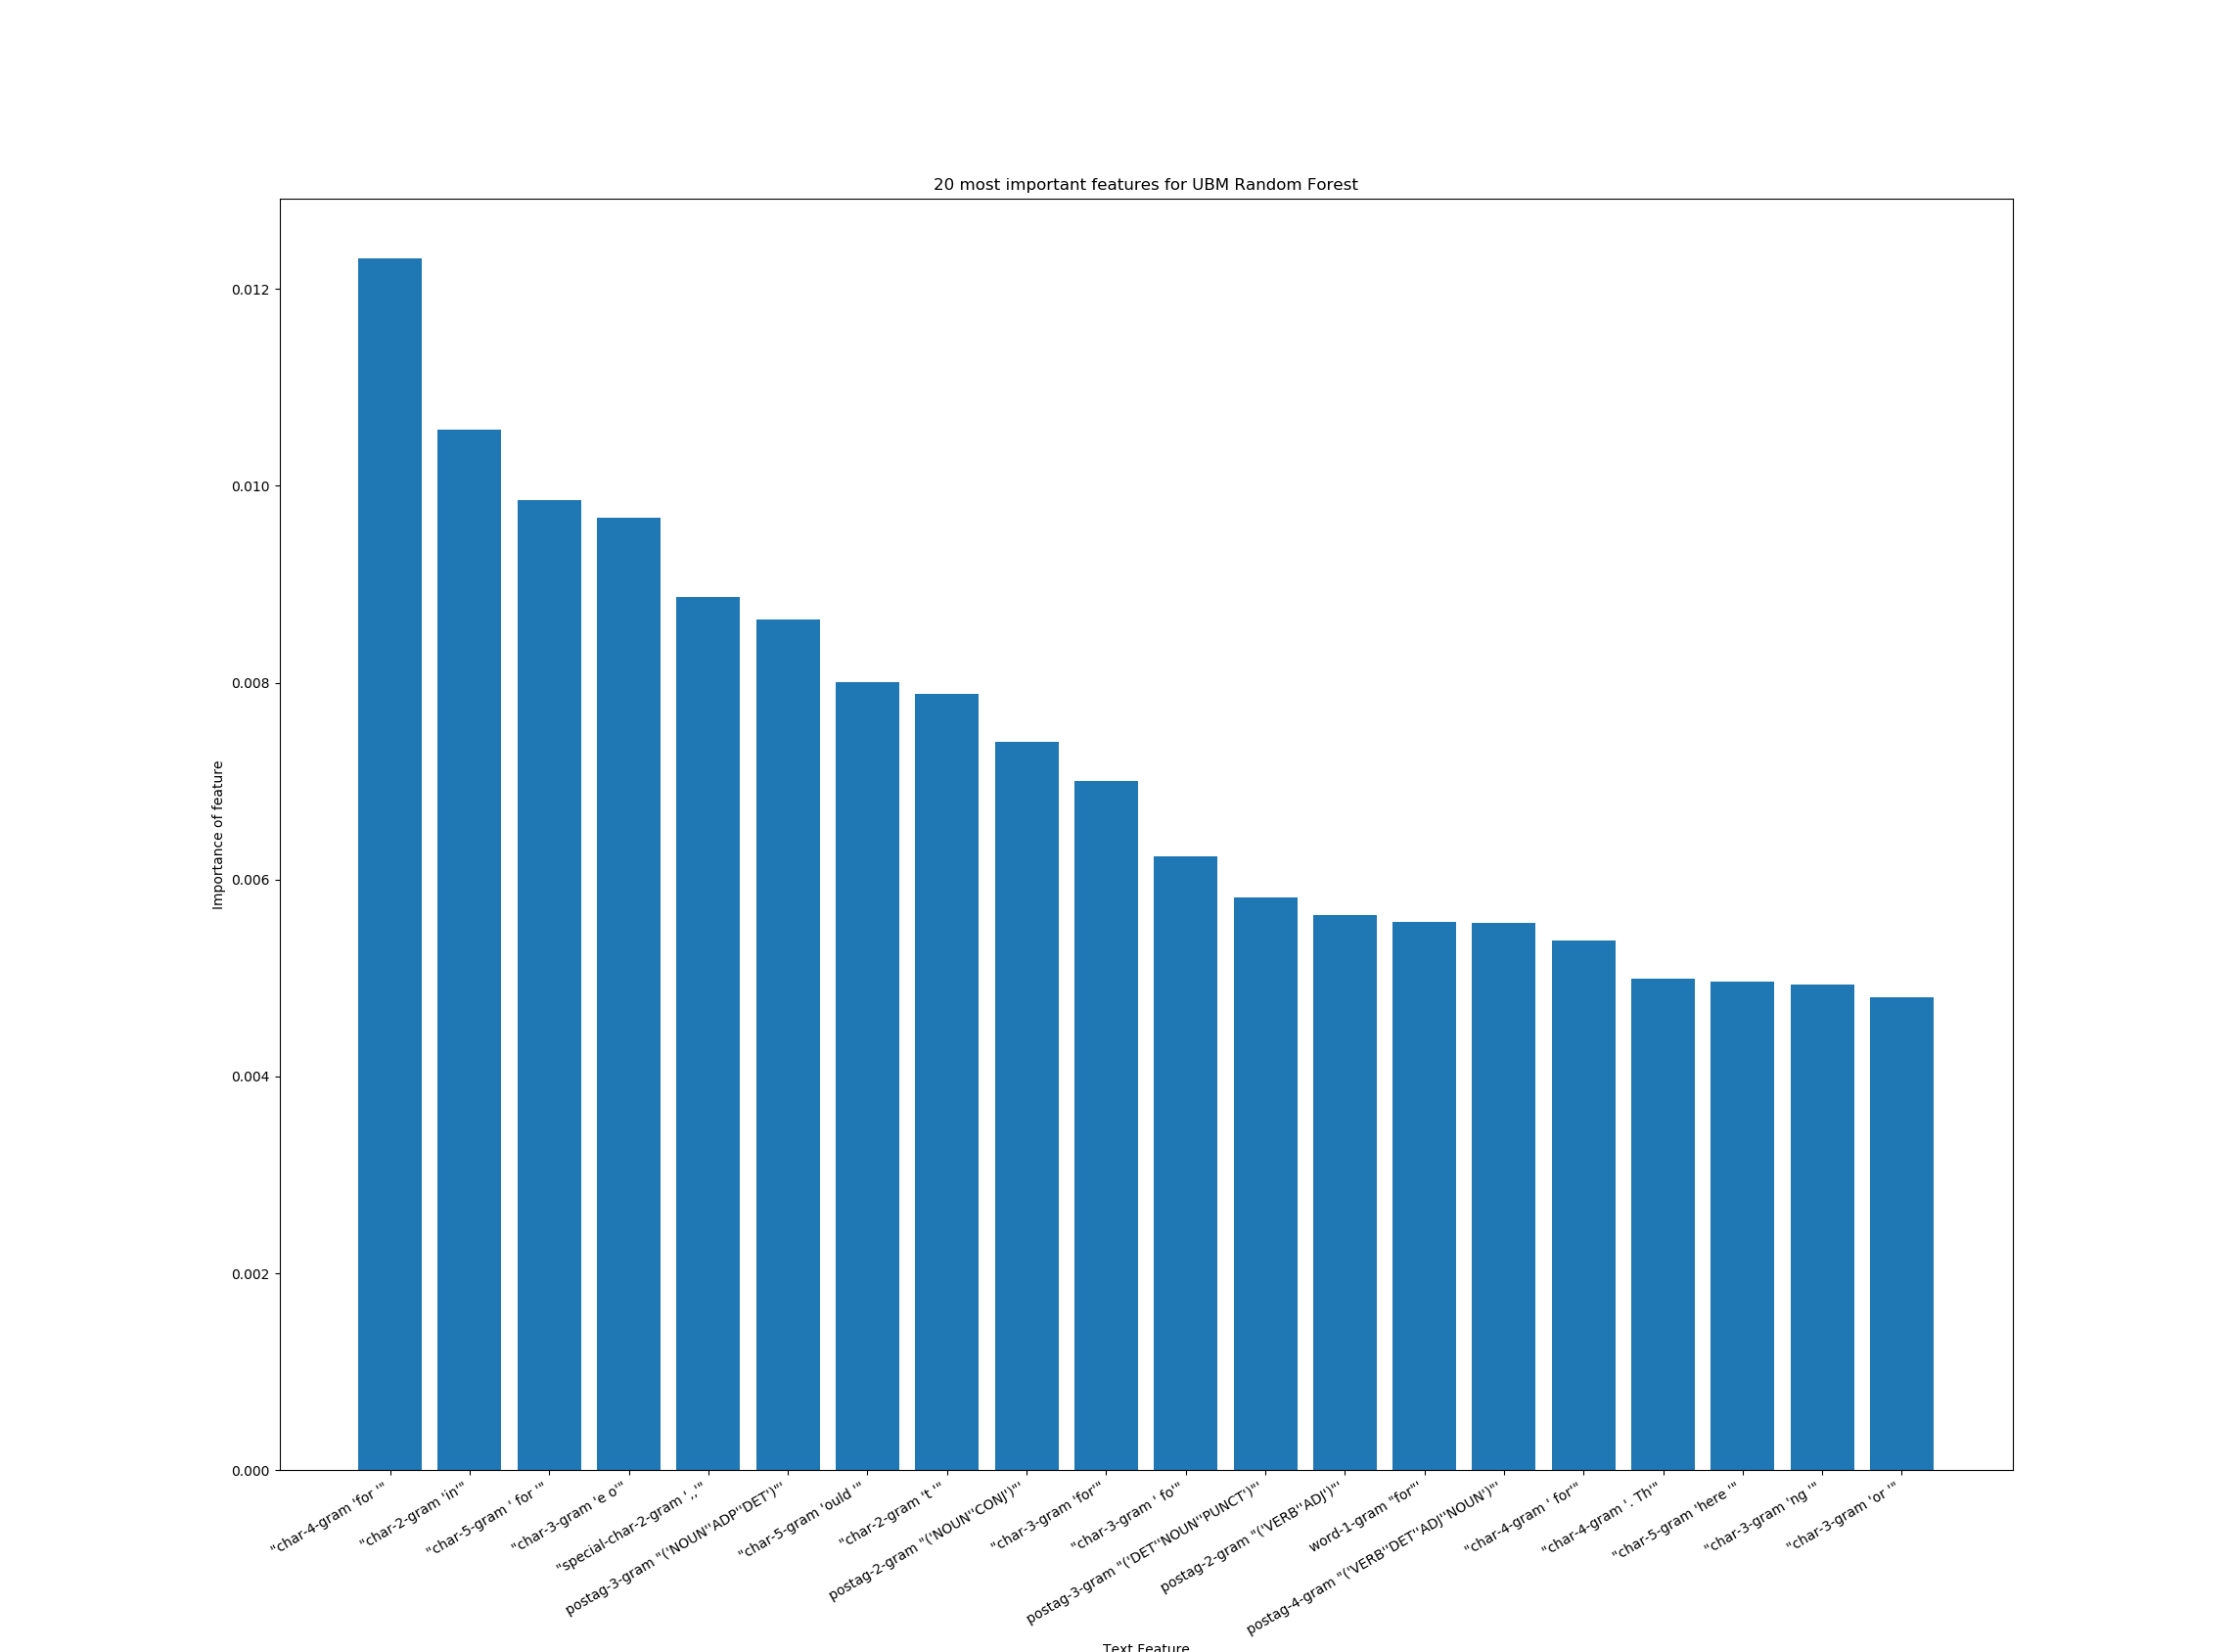
\includegraphics[scale=.34]{./pictures/FeatureImpotrance20.png}
        \caption{The 20 most important features after applying the UBM encoded
        features to the random forest model}
        \label{fig:feature_importance_small}
    \end{figure}
\end{landscape}

\begin{figure}
    \centering
    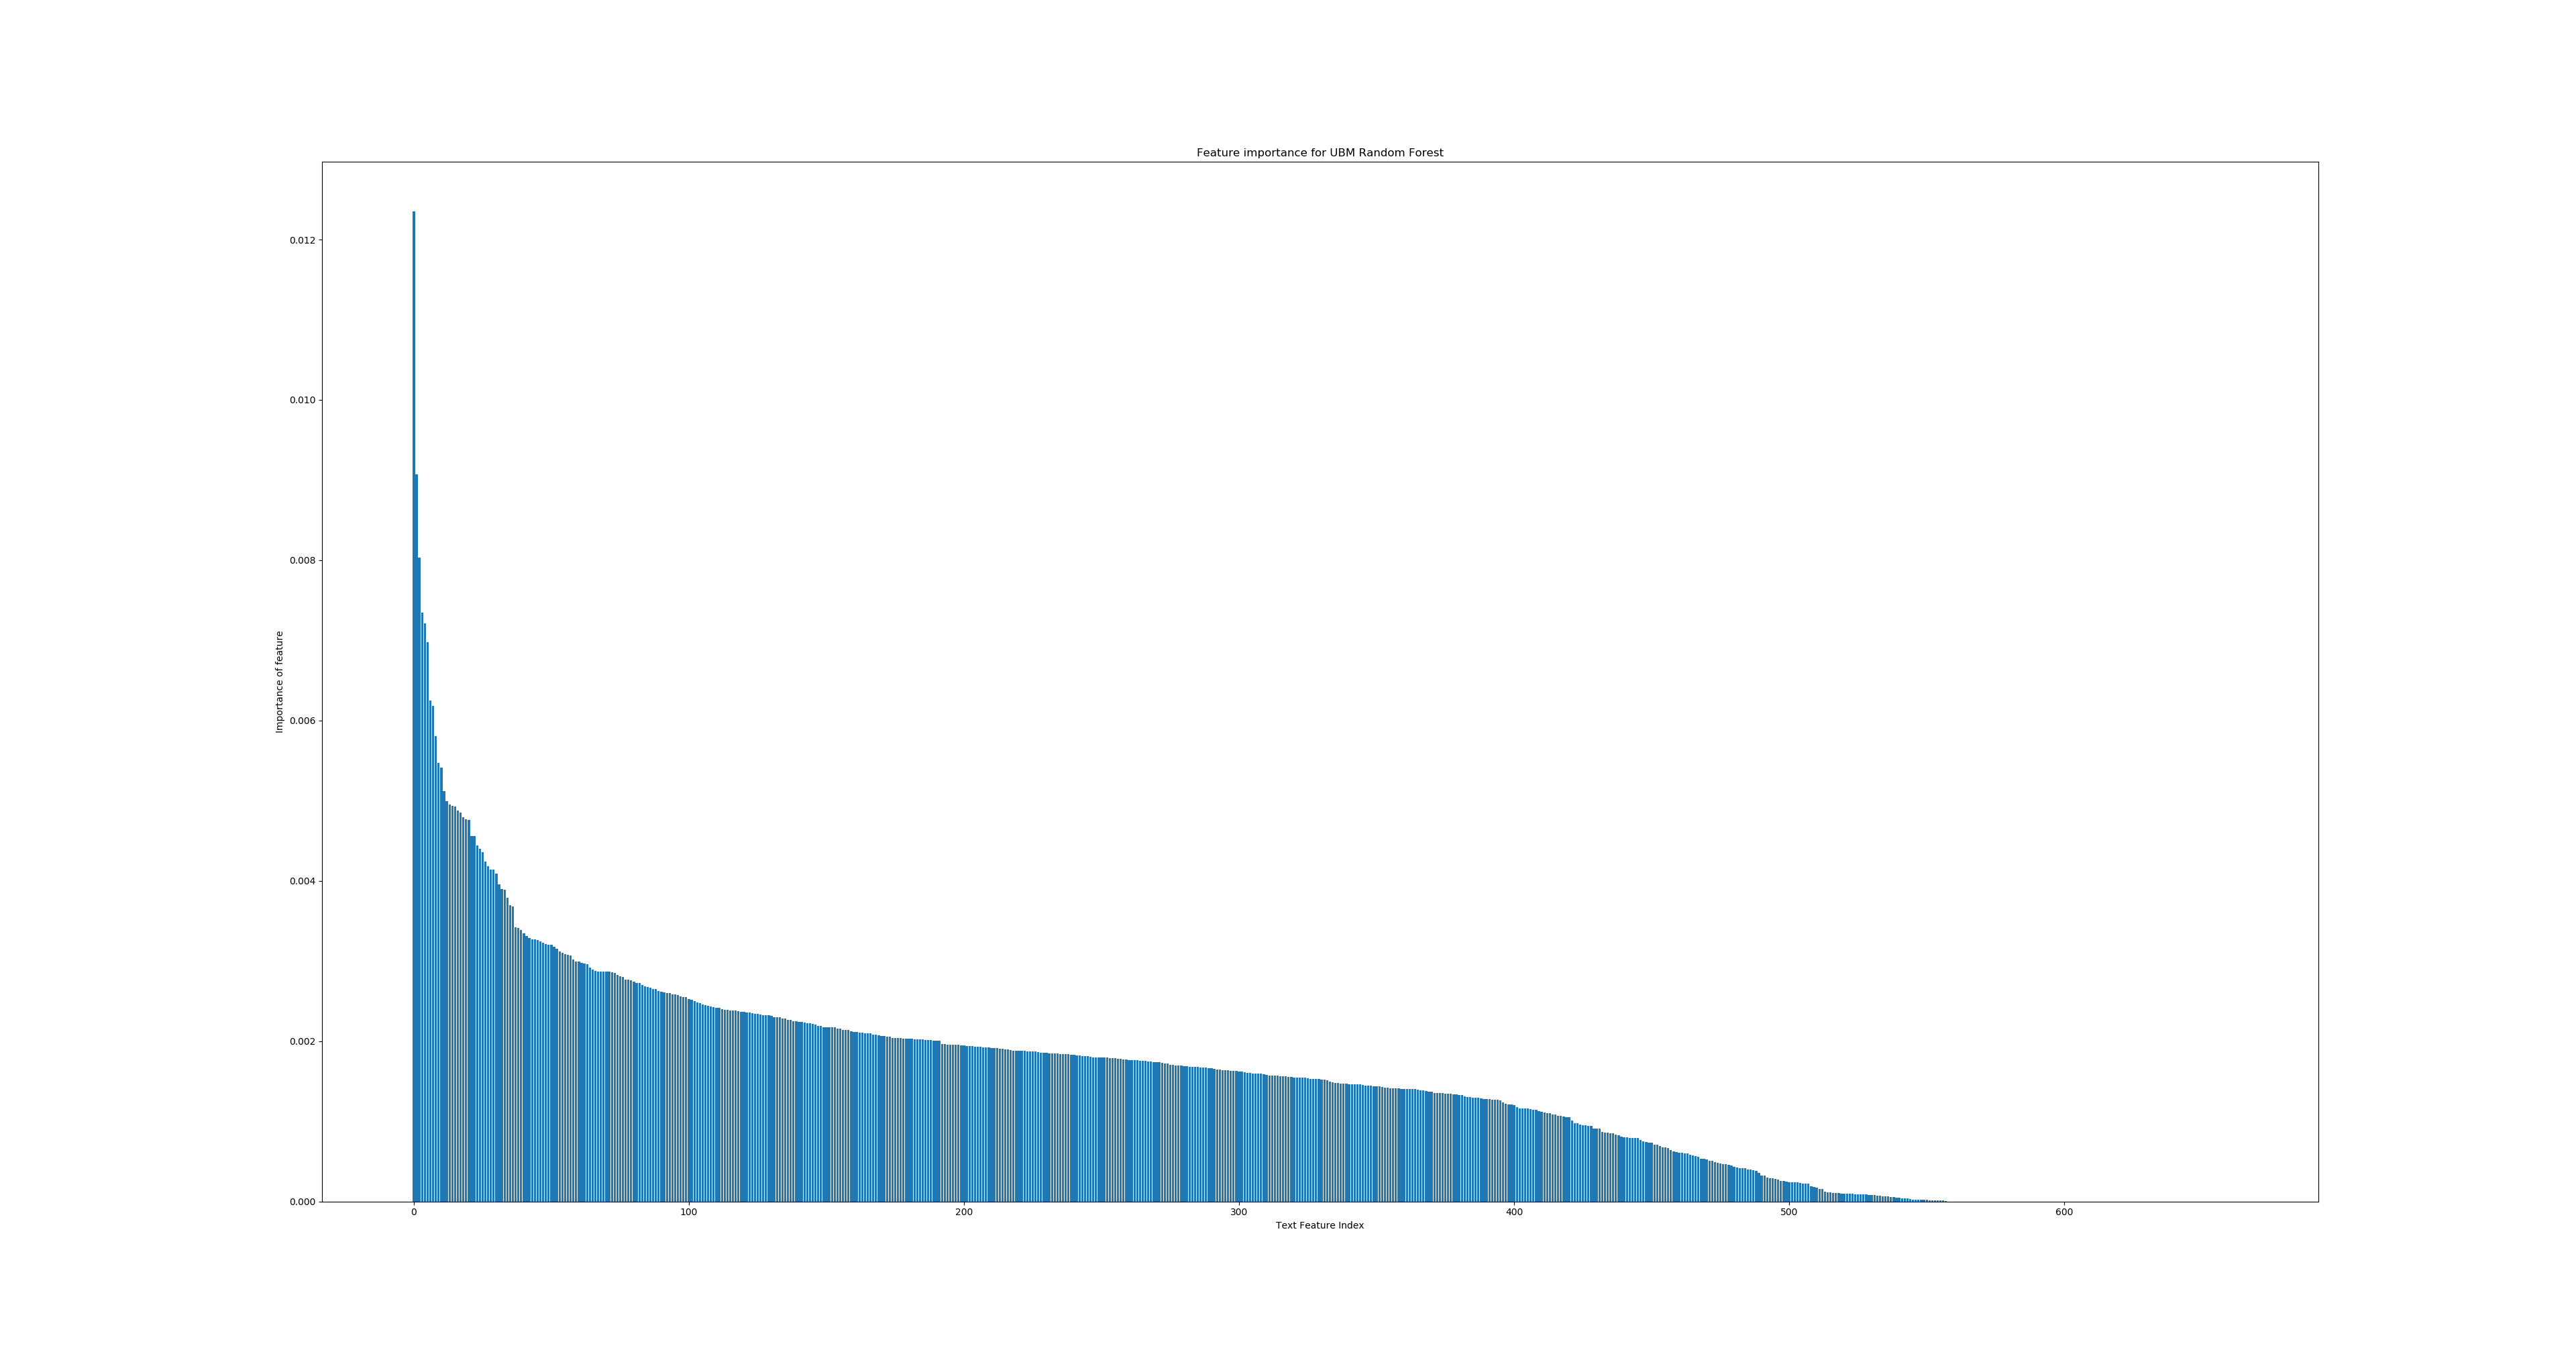
\includegraphics[scale=.34]{./pictures/FeatureImpotranceAll.png}
    \caption{The feature importance for all UBM encoded features given
    to the random forest model on the PAN 2015 dataset.}
    \label{fig:feature_importance_all}
\end{figure}

From that overview it is clear that the most important feature is the frequency
of the word \textit{for} as multiple features seem to capture that word. Most
of the words captured by the different features seem to be English stop words.
Both \textit{for}, \textit{in}, \textit{could}, \textit{should}, \textit{would},
\textit{here} and \textit{or} seem to be represented in the list and are part
of the list of English stop words \footnote{https://www.ranks.nl/stopwords}.
Besides that an important feature is the special-character-2-gram consisting
of two commas. That feature might capture an authors tendency to using long
sentences. Longer sentences will more likely contain a larger amount of commas.
The character-4-gram ". Th" most likely captures an authors tendency to start
her sentences with the word "The". Besides that the \gls{POS}-tags capture the
general sentence structure of the authors.

The reason the English stop words are so important is probably because they are
consistently used over all genres. Texts about different topics and in different
genres will probably all contain the words \textit{the} and \textit{for}. It
is therefore easier to use them as an estimate of which author has written the
text since they are not dependent on which genre or type of text the author was
writing.

The least important features according to the random forest are shown in
Table \ref{tab:feature_non_importance}. That all of those features consist of
word-5-grams and all of them seem to be very specific to a source text. For
example one of the features are the words "in the united states and". There is a
good chance that no author will have that phrase at about the same frequency in
all texts she writes. The phrase will clearly be more prevalent in texts about
the United States and less prevalent in cooking recipes even though they have
the same author.

\begin{table}
    \centering
    \begin{tabular}{lll}
        \textbf{Feature Class} & \textbf{Feature} & \textbf{Importance Score} \\
        \hline
        word-5-gram & is one of the most                  & 0.0 \\
        word-5-gram & index words and electronic switches & 0.0 \\
        word-5-gram & in the united states and            & 0.0 \\
        word-5-gram & at the foot of the                  & 0.0 \\
        word-5-gram & we are born of god                  & 0.0 \\
        word-5-gram & turned out to be a                  & 0.0 \\
        word-5-gram & the state of rhode island           & 0.0 \\
        word-5-gram & the secretary of the interior       & 0.0 \\
        word-5-gram & the second half of the              & 0.0 \\
        word-5-gram & the first half of the               & 0.0 \\
        word-5-gram & the far end of the                  & 0.0 \\
        word-5-gram & president of the united states      & 0.0 \\
        word-5-gram & of the state of rhode               & 0.0 \\
        word-5-gram & of the government of the            & 0.0 \\
        word-5-gram & if we are born of                   & 0.0 \\
        word-5-gram & for the rest of the                 & 0.0 \\
        word-5-gram & for a number of years               & 0.0 \\
        word-5-gram & at the time of the                  & 0.0 \\
        word-5-gram & are born of god we                  & 0.0 \\
        word-5-gram & year of our lord one                & 0.0
    \end{tabular}
    \caption{The 20 features the random forest least often split on when doing
    authorship verification on the PAN 2015 dataset.}
    \label{tab:feature_non_importance}
\end{table}

It was not only word-5-grams that did not perform very well. After training our
random forest model, it became apparent that in no case did word n-grams perform
well. The reason for that might be the lack of text in the PAN 2015 dataset.
The texts on PAN 2015 being limited to an average of 460 words meaning that
there are few different word-n-grams in the texts. However, the word-n-grams
extracted from the brown corpus vary a lot and is usually very subject specific
as described above. As such only a few of the word-n-grams extracted from the
brown corpus are in the PAN 2015 texts. This only becomes more evident as n
increases as the word-n-grams becomes more and more text specific.

Looking at figure \ref{fig:feature_importance_all} however, we can see that
the overall feature contribution is somewhat good. Based on the fact that
600 features were used, meaning that each feature importance averages out at
$\frac{1}{600} = 0.00166666666$ if the importance was equally distributed, which
is represented as a line on the graph. As such rather than our model depending
on a very small amount of features, it can be seen that
over 50\% of the feature set actually contributes to the classification, with
an importance over the average. While this could very well only be the case for
our selected features, it does lend some credence to the idea that using more
features in the forest during training could increase accuracy.

\subsection{Performance of our different methods}

The Delta Method was our baseline method and has been found to perform well in
the authorship verification setting \cite{evert2015towards}. On the PAN 2013
datasets we obtained an average accuracy of 0.62252 which is not a significant
result, compared to the other results on the 2013 set. From the average
\gls{TPR} (0.52196) and \gls{TNR} (0.71204) we can see that the main problem is
the \gls{TPR}. When the \gls{TPR} is low we have a large number of \gls{FN}s
compared to \gls{TP}s which means that we will often say a text is written by a
different author even though it is written by the same author. On the training
data we found that the number of opposing authors on the 2013 dataset should be
4 but it seems like the number was to high for the test dataset. Even though the
results were not significant we still ranked 13/19 when comparing to the other
competitors that year. On the PAN 2015 dataset we obtained a final score of
0.34201 an \gls{TPR} of 0.54899 and a \gls{TNR} of 0.60800. Again the \gls{TNR}
is far better than the \gls{TPR}.

The Generalized Random Forest was off to a bad start start, as the paper it
was based on \cite{pacheco2015} only got 6'th place in the PAN 2015 authorship
verification task, and our implementation of that same method only ranked 9'th.
The main focus of this method however, was the way it attempted to circumvent
the lack of data, associated with each specific author, by instead learning
on the author-known texts dataset in its entirety. While the results of this attempt
didn't land us at any place near the top, in terms of placement it did work. By
comparing our \gls{UBM} based results to the author specific Minus encoding we
can see an improvement in terms of accuracy, thus making the \gls{UBM} a viable
choice when faced with small amounts of entry-specific data. We only ran the
method on the PAN 2015 dataset where it got a score of 0.38576 for \gls{UBM} and
0.33183 for Minus. Opposite to the Delta Method the main problem of the forest
is not the \gls{TPR} but the \gls{TNR}. The rates obtained were \gls{TPR} of
0.63200 for \gls{UBM} and 0.66800 for Minus and \gls{TNR} of 0.57600 and 0.50000
for Minus. 

The Extended Delta Method achieved the best result of any of our methods on
the PAN 2015 data. The ROC curve for the method is clearly the best one of
any of our implemented methods. On the PAN 2013 dataset it used a collection
of different features while on the PAN 2015 dataset the method used only 60
features and all of them were different special-character-n-grams. We tried the
method using both the Euclidean and the Manhattan distance. They performed about
the same but the Manhattan distance was a little better in all cases. Which
is similar to the findings of \cite{evert2015towards}. In general Manhatten
distances emphasises the differences over more small features instead of single
large ones so it seems like it is important to consider the differences in many
features when doing authorship verification. The method obtained an accuracy
of 0.69909 on the PAN 2013 dataset and final score of 0.40383 on the PAN 2015
dataset. Both results are significant improvements over the original Delta
Method we also tried. The \gls{TPR}s were 0.71255 for PAN 2013 and 0.49760 for
PAN 2015 and the \gls{TNR}s were 0.68098 for PAN 2013 and 0.74140 for PAN 2015.
It seems like the PAN 2013 method is good both at identifying when texts are
written by the same author and when they are not while the PAN 2015 method is
only good at identifying when texts are written by different authors.

The Author Specific SVM performed very well on the PAN 2013 dataset. As
described by \cite{stamatos2009} \gls{SVM}s are great for doing Authorship
Attribution and Verification since they are able to handle very large amounts of
features. And since representing a text document will typically use very large
vectors \gls{SVM}s are a natural approach. Besides the accuracy the \gls{TPR}
and \gls{TNR} achieved by the Author Specific SVM was also very good. However
they were clearly better on the training dataset than on the testing dataset.
The main drawback of the SVM method is that it requires either several examples
of text from an author or a single long example that can be split into multiple.
\cite{stamatos2009} describes that performance for \gls{SVM}s have previously
been shown to drop significantly when only a small amount of data is available.
Unfortunately the PAN 2015 dataset did not contain enough data for us to split
the text into multiple and try the SVM approach on them. The accuracy, \gls{TPR}
and \gls{TNR} obtained were 0.77858, 0.71114 and 0.83582. The results are
excellent, the \gls{SVM} are both good at finding when texts are written by the
same author and when they are written by different authors.

\subsection{Improvements}

While the Random Forest method didn't provide any impressive results, the
generalized approach might very well be useful in the future, in case one comes
across another sparse dataset. An improvement could be to increase the number
of features fed to the random forest. Not only quantity, but also different
types of features than the ones used in this paper. This would work since Random
Forest by its very nature selects the best features for classification. Thus we
can, at the cost of some run time, train on a much larger feature-set and we
suspect that this better results might be produced, a point supported by Figure
\ref{fig:feature_importance_all} as mentioned earlier.

Similar to the Random Forest method the Author Specific SVM might also have been
able to perform better by using more features. As explained earlier \gls{SVM}s
are very good at handling large amounts of features so we could have probably
improved performance by adding more. Furthermore as described earlier the
solutions that performed better than ours usually used extra text documents not
from the dataset as opposing authors (imposters). We believe that we might have
achieved better results if we had done that too.

We could have also tried more distance metrics/measures in the extended Delta
Method. The Cosine Measure has by \cite{evert2015towards} been shown to perform
better than the Manhattan distance. We could have also tried the Min/Max measure
which \cite{aalykke2016} found to be the best distance metric/measure for Danish
texts.
